\documentclass[tikz,border=10pt]{standalone}
\usepackage{tikz}
\usepackage{xcolor}

\definecolor{hse-hellblau}{cmyk}{.75,.1,.06,0}
\definecolor{hse-blau75}{HTML}{8abde2}
\definecolor{hse-blau50}{HTML}{b4d3ed}
\definecolor{hse-blau25}{HTML}{dbe9f7}
\definecolor{hse-blau15}{HTML}{eaf2fa}
\definecolor{hse-hellgrau}{cmyk}{0,0,0,.08}

\begin{document}
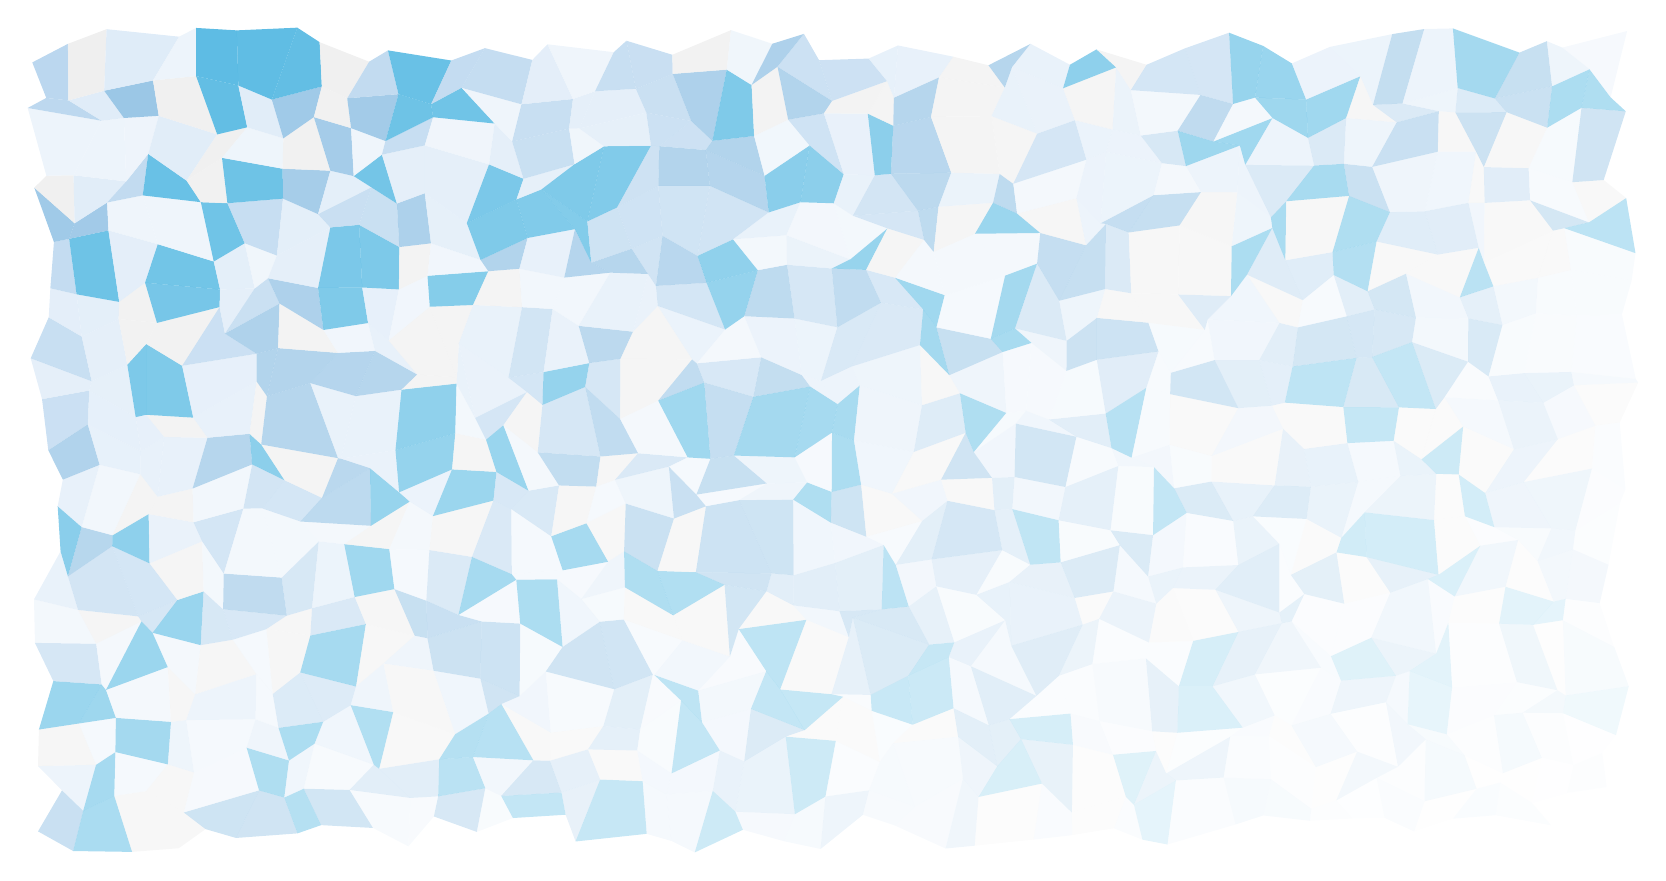
\begin{tikzpicture}[scale=0.5]
    \pgfmathsetseed{1}  % Setze einen Seed für Reproduzierbarkeit
    
    % Erstelle ein Raster von Punkten mit zufälligen Verschiebungen
    \foreach \i in {0,...,40} {
        \foreach \j in {0,...,20} {
            \pgfmathsetmacro\dx{rand*0.5}
            \pgfmathsetmacro\dy{rand*0.5}
            \coordinate (p-\i-\j) at ({\i+\dx}, {\j+\dy});
        }
    }
    
    % Zeichne die Polygone
    \foreach \i in {0,...,39} {
        \foreach \j in {0,...,19} {
            \pgfmathsetmacro\rand{int(random(0,5))}
            \pgfmathsetmacro\opacity{1 - (0.1 + 0.9*(\i+2*(19-\j))/78)}
            
            \ifcase\rand
                \def\cellcolor{hse-hellblau}
            \or
                \def\cellcolor{hse-blau75}
            \or
                \def\cellcolor{hse-blau50}
            \or
                \def\cellcolor{hse-blau25}
            \or
                \def\cellcolor{hse-blau15}
            \or
                \def\cellcolor{hse-hellgrau}
            \fi
            
            \pgfmathtruncatemacro\nextI{\i+1}
            \pgfmathtruncatemacro\nextJ{\j+1}
            
            \fill[\cellcolor, opacity=\opacity] 
                (p-\i-\j) -- (p-\nextI-\j) -- (p-\nextI-\nextJ) -- (p-\i-\nextJ) -- cycle;
        }
    }
\end{tikzpicture}
\end{document}